\section{Evaluation}
\label{eval}
We have implemented the BLSCoSi protocol described in Section \ref{design} in Golang and made it available on Github \footnote{At \hyperlink{BLSFTCoSi}{https://github.com/dedis/student\_18\_blsftcosi}}. For BLS signatures we use the bilinear bn256 \cite{bn256}  group of elliptic curves. We evaluated it on Deterlab\cite{deterlab} using upto 20 physical machines with 16 GB RAM to simulate upto 1,000 CoSi witnesses. The simulated network was set with a roundtrip delay of 5 milliseconds on a 1GBps link between the physical servers. We used a 3-level tree-structure with $O(\sqrt{n})$ branching factor. Acceptance threshold was set to $2f +1$ on the network of $3f$ nodes to simulate a Byzantine-fault tolerant system that can tolerate upto $f$ malicious nodes. In Figure \ref{fig}, we evaluate scalability of BLSCoSi under different block sizes and failure rates. 

\subsection{Scalability}
 For BLSCoSi rounds with 0\% failures in Figure \ref{fig}, we observe a linear increase in latency with increasing number of nodes. The latency also doubles with doubling the block-size, confirms linear increase for the same. Signing 8 MB block on BLS-Cosi can account can incur latency $\sim$3 sec with 1k cosigners.

Compared with Flat-BLS which is a 2-level tree-structure where only the root performs all the aggregations, we see that increasing the block-size can exponentially increase the latencies as the aggregations cost at the root is affect by both the size of the signature and the number of signatures.

\subsection{Fault tolerance}
We simulated node failures in BLSCoSi by randomly choosing x\% nodes to become unresponsive during the protocol run. For the experiment we ran 10 rounds of the protocol and averaged their latencies. The BLSCoSi protocol with 10\% and 20\% failures sees an increase of 2.5x and 4x in the latencies. While the failures at the leaf nodes does not affect the protocol, the failures at the subleader makes the signatures from the entire subtree unavailable. Subleader-change is triggered only through timeout and the current timeout (5 sec for the protocol, 2.5 sec for the sub-protocol) on the  BLSCoSi allows for only a single subleader change. In the cases where the subsequent subleaders of a subtree are unresponsive, in the entire subtree fails to participate in the cosigning round. 

\subsection{Comparison with CoSi}
We evaluated CoSi on a similar tree structure as BLSFTCoSi with 0\% failures. The smaller block-sizes (< 1 MB) showed smaller latencies for BLSCoSi but for a larger block-size of 4 MB, showed better latency for CoSi. This can be attributed to the fact the BLS signatures are computationally much more intensive than ECDSA signatures. With larger block sizes and larger number of nodes in BLSCoSi, the computational latencies likely overtake the commmunication latencies. This can also be seen from the fact that the latency graph for BLSCoSi gets much more steeper with block-size increase than the same for CoSi.

\begin{figure}[h]
	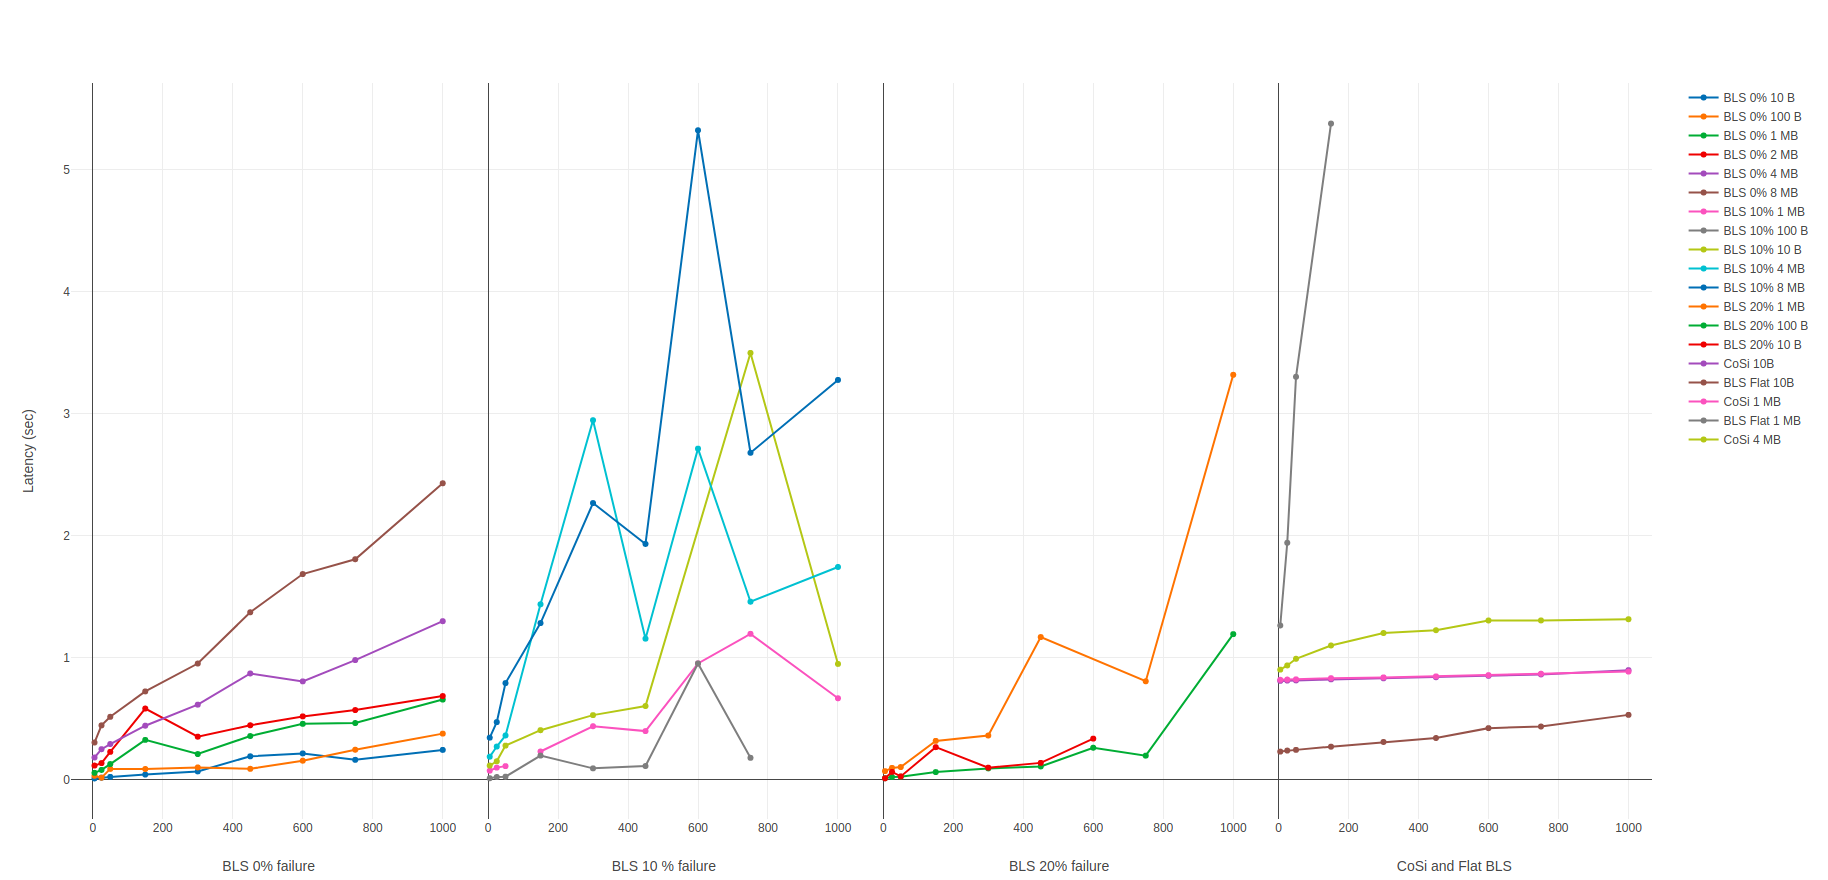
\includegraphics[angle=90,width=10cm]{all.png}
	\caption{Latency of BLSCoSi round under different scenarios}
	\label{fig}
\end{figure}
\clearpage